\documentclass[12pt,letterpaper]{article}

\usepackage[hypertexnames=false]{hyperref}
\usepackage{amsmath}
\usepackage{graphicx}
\usepackage{enumerate}

% Custom packages
\usepackage{amssymb}
\usepackage{booktabs}       % professional-quality tables
\usepackage{algorithm}      % algorithm environment
\usepackage{algpseudocode}
\usepackage{multirow}
\usepackage{sectsty}
\usepackage{tabularx}
\usepackage{tikz}           % vector graphics
\usepackage{bm}             % bold math symbols
\usepackage{xcolor}
\usepackage{microtype}
\usepackage{import}
\usepackage{titling}
\usepackage{natbib}
\usetikzlibrary{arrows, backgrounds, patterns, matrix, shapes, fit, 
  calc, shadows, plotmarks}


% Custom commands
\let\oldvec\vec
\renewcommand\vec{\bm}
\newcommand{\simfn}{\mathtt{sim}} % similarity function
\newcommand{\truncsimfn}{\underline{\simfn}} % truncated similarity function
\newcommand{\blockfn}{\mathtt{BlockFn}} % blocking function
\newcommand{\distfn}{\mathtt{dist}} % distance function
\newcommand{\valset}{\mathcal{V}} % attribute value set
\newcommand{\entset}{\mathcal{R}} % set of records that make up an entity
\newcommand{\partset}{\mathcal{E}} % set of entities that make up a partition
\newcommand{\1}[1]{\mathbb{I}\!\left[#1\right]} % indicator function
\newcommand{\euler}{\mathrm{e}} % Euler's constant
\newcommand{\dblink}{\texttt{\upshape \lowercase{d-blink}}} % Name of scalable Bayesian ER model
\newcommand{\blink}{\texttt{\upshape \lowercase{blink}}} % Name of original Bayesian ER model
\def\spacingset#1{\renewcommand{\baselinestretch}%
  {#1}\small\normalsize} \spacingset{1}

\newtheorem{remark}{Remark}
\newtheorem{proposition}{Proposition}
\newtheorem{definition}{Definition}
\newtheorem{lemma}{Lemma}
\def \brian#1{{\color{red} (#1)}}

% DON'T change margins - should be 1 inch all around.
\addtolength{\oddsidemargin}{-.5in}%
\addtolength{\evensidemargin}{-.5in}%
\addtolength{\textwidth}{1in}%
\addtolength{\textheight}{1.3in}%
\addtolength{\topmargin}{-.8in}%

\sectionfont{\large\nohang\centering\MakeUppercase}

\title{Bayesian Matching for Possible Internal Duplications through Dirichlet Record Linkage}
\author{Brian Kundinger}

\begin{document}
%\maketitle
%
%\bigskip
%\begin{abstract}
%Abstract
%\end{abstract}
%
%\newpage
\spacingset{1.5}

%\section{Introduction}

%There have been several other attempts to estimate more flexible linkage structures within the comparison vector framework, but each has significant drawbacks in practice. First, the original \cite{fellegi_theory_1969} method that models the linkage status of each record pair as independent typically results in one record in one file being matched with multiple records in the other file. This initial estimate of the linkage structure is usually refined through post-processing to create a bipartite matching \cite{jaro1989}. As of yet, this post-processing has not been adapted to estimate more general linkage structures, and the initial estimate without any post-processing is known to have poor precision. \cite{aleshinguendel2021multifile} allowed for multiple matches within and across datafiles, but requires that the modeller explicitly set a maximum linkage cluster size, and models the dependency between records in such a way that limits scalability. \cite{zanella_flexible_2016} used nonparametric priors for the number of unique entities in a record linkage task, and showed that this doesn't work. TODO.

%In contrast, we propose a nonparametric distribution for the number of matches that each record in one datafile has in the other datafile. In SECTION, we introduce this approach as an extension  of \texttt{fabl} method, and in SECTION, show how it can be adopted within the \texttt{vabl} framework as well. We demonstrate the effectiveness of this method through several simulations and case studies. 
%\section{Review of fabl}
%
%The full model for fabl is given by:
%
%\begin{subequations}
%	\begin{align}
%		\mathcal{L}(Z, \bm{m}, \bm{u} \mid \gamma) &= \prod_{i=1}^{n_A}  \prod_{j=1}^{n_B}\prod_{f=1}^{F}\prod_{l=1}^{L_f}\left[  m_{fl}^{I(Z_j = i)}u_{fl}^{I(Z_j \neq i)}\right]^{I(\gamma_{ij}^f = l)I_{obs}(\gamma_{ij}^f)}, \label{eqn:likelihood}\\
%		\bm{m}_f &\sim \text{Dirichlet}(\alpha_{f1}, \ldots, \alpha_{f L_f}), \forall f = 1, \ldots, F, \label{eqn:m} \\
%		\bm{u}_f &\sim \text{Dirichlet}(\beta_{f1}, \ldots, \beta_{f L_f}),\forall f = 1, \ldots, F,  \label{eqn:u}\\
%		p(Z_j = q| \pi)  &=
%		\begin{cases} 
%			\frac{1}{n_A}\pi,  & q > 0; \\
%			1-\pi, &  q  = 0; \\
%		\end{cases} \label{eqn:z}\\
%		\pi &\sim \text{Beta}(\alpha_{\pi}, \beta_{\pi})\label{eqn:pi}.
%	\end{align}
%\end{subequations}

%\section{Motivation}
%
%We have shown in previous work that the fast Beta linkage framework tends to outperform standard Fellegi Sunter when each record in $B$ has at most one match in $A$. However, significant problems arise when a record in $B$ has multiple matching records in $A$. In particular, since matching probability is normalized among all records in $A$, matching probability is split among multiple records such that none of the matches achieves high enough posterior probability to be identified through the Bayes estimate. This amounts to a paradox: the more matches that record $B_j$ has in $A$, the less likely the algorithm is to find a match. 
%
%We attempt to resolve this paradox by extending the fabl framework to handle these internal duplications. We introduce a modified Dirichlet process prior that allows each record in $B$ to match to potentially multiple records in $B$. We emphasize that we are not interested in deduplication within either dataset for its own sake, but rather aim to conduct record linkage in light the problems posed by these duplications. For this reason, we do not enforce transitive closure throughout the Gibbs sampler as done in \cite{marchant_distributed_2019} and \cite{aleshinguendel2021multifile}, but rather assume it, and create a coherent set of linkages through post-processing. This allows for a record linkage model that is robust to internal duplications while maintaining the computational advantages of the original \texttt{fabl} model. 

\section{Dirichlet Record Linkage}

Recall that for \texttt{fabl}, we used the following prior for the linkage structure $Z$ and the rate of matching parameter $\pi$:
\begin{subequations}
	\begin{align}
		p(Z_j = q| \pi)  &=
		\begin{cases} 
			\frac{1}{n_A}\pi,  & q > 0; \\
			1-\pi, &  q  = 0; \\
		\end{cases} \label{eqn:fabl_prior}\\
		\pi &\sim \text{Beta}(\alpha_{\pi}, \beta_{\pi})\label{eqn:pi_beta}.
	\end{align}
\end{subequations}
This prior says that a record $B$ has some match in $A$ with probability $\pi$, and that each record in $A$ is equally likely to be that match. We now generalize these prior distributions to allow the records in $B$ to match with multiple records in $A$. 

\subsection{Prior Specification}\label{sec:prior-specification}

We provide updated notation to allow us to describe one record in $B$ having multiple matches in $A$. Let $Z_j$ be a set containing the indices for all of the records in $A$ that are a match with record $B_j$, and let $Z = \{Z_j | j = 1, \ldots, n_B\}$ denote the collection of such sets for all records in $B$. Let $|Z_j| = \sum_{k=1}^{\infty} I(Z_{j, k} > 0)$ denote the number of records in $A$ that are linked to $B_j$. We use $Z_j = \emptyset$ to denote when $B_j$ has no match in $A$.

We modify the \texttt{fabl} model to allow each record in $B$ to match to multiple records in $A$. Define a vector of probabilities $\bm{\pi} = (\pi_0, \ldots, \pi_{n_A})$ where $\pi_k$ is the probability that some record in $B$ has exactly $k$ matches in $A$. Conditional on $B_j$ having $k$ matches, we construct a prior specification on $Z$ such that each matching $Z_j$ of length $|Z_j|$ is equally likely. Since there are ${n_a \choose |q|} = \frac{n_A!}{(n_A - |q|)! |q|!}$ ways to select $|q|$ matching records out of all $n_A$ possible records, we replace (\ref{eqn:fabl_prior}) with
\begin{align}\label{eqn:z}
	p(Z_j = q| \bm{\pi}) = \frac{(n_A - |q|)! |q|!}{n_A!} \pi_{|q|}.
\end{align}
Since $\pi$ is multivariate, we replace (\ref{eqn:pi_beta}) with
\begin{align}
	\bm{\pi}\sim \text{Dirichlet}(\alpha_{\pi}).
\end{align}
%Similar to fabl, we adopt a prior specification on $Z$ so that each matching $Z_j$ of length $|Z_j| = k$ is equally likely. Since there are $n_a \choose |q| = \frac{n_A!}{(n_A - |q|)! |q|!}$ ways to select $|q|$ matching records out of all $n_A$ possible records, we use
%\begin{align}\label{eqn:z}
%	p(Z_j = q| \bm{\pi}) = \frac{(n_A - |q|)! |q|!}{n_A!} \pi_{|q|}.
%\end{align}

%where the additional $|q|!$ accounts for the multiple orderings of $q$. Though the representation in (\ref{eqn:z_equivalence}) is more natural in the record linkage settings, the representation in (\ref{eqn:z}) will provide more clear derivations in the sections that follow. 
%Similar to fabl, we adopt a prior specification on $Z$ so that each matching $Z_j$ of length $|Z_j| = k$ is equally likely. Formally, we have
%
%\begin{subequations}
%	\begin{align}
%		\mathcal{L}(Z, \bm{m}, \bm{u} \mid \gamma) &= \prod_{i=1}^{n_A}  \prod_{j=1}^{n_B}\prod_{f=1}^{F}\prod_{l=1}^{L_f}\left[  m_{fl}^{I(i \in Z_j)}u_{fl}^{I(i \notin Z_j)}\right]^{I(\gamma_{ij}^f = l)I_{obs}(\gamma_{ij}^f)}, \label{eqn:likelihood}\\
%		\bm{m}_f &\sim \text{Dirichlet}(\alpha_{f1}, \ldots, \alpha_{f L_f}), \forall f = 1, \ldots, F, \label{eqn:m} \\
%		\bm{u}_f &\sim \text{Dirichlet}(\beta_{f1}, \ldots, \beta_{f L_f}),\forall f = 1, \ldots, F,  \label{eqn:u}\\
%%		p(Z_j = q| \bm{\pi})  &=
%%		\begin{cases} 
%%			\frac{(n_A - k)! k!}{n_A!} \pi_k,  & q \neq 0, \\
%%			\pi_0, &  q  = 0; \\
%%		\end{cases} \\
%		p(Z_j = q| \bm{\pi}) &= \frac{(n_A - |q|)! |q|!}{n_A!} \pi_{|q|}
% \\
%		\pi_k &= (1 - \eta_{k+1}) \prod_{c=1}^{k} \eta_c,  \\
%		\eta_k &\sim \text{Beta}(\alpha_{\eta}, \beta_{\eta})\label{eqn:pi}.
%	\end{align}
%\end{subequations}


%Below, we explain how this prior is implemented in the MCMC and variational inference frameworks, and the computational considerations relevant to each. 
%MAKE MORE FORMAL.

\subsection{Full Conditional for $Z_j$}\label{sec:joint-distribution}

Following the observation of \cite{wortman2019} and elaborated by \cite{kundinger_2023}, when $B_j$ does not link to any record in $A$ (such that $|Z_j| = 0$) the contribution to the likelihood is simply a product of $u$ parameters, which we will call $c_j$:
\begin{align}
	p(\Gamma_{.j}| \bm{m}, \bm{u}, \pi, Z_j = \emptyset) = \prod_{i=1}^{n_A}\prod_{f=1}^{F}\prod_{l=1}^{L_f} u_{fl}^{I(\gamma_{ij}^f = l)I_{obs}(\gamma_{ij}^f)} = c_j.
\end{align}
When $Z_j = q =  (q_1, \ldots, q_k)$ for some $|q| > 0$, we have
\begin{align}
	p(\Gamma_{.j}| \bm{m}, \bm{u}, \pi,  Z_j = q) =\prod_{i \in q}\prod_{f=1}^{F}\prod_{l=1}^{L_f} m_{fl}^{I(\gamma_{ij}^f = l)I_{obs}(\gamma_{ij}^f)}  \prod_{i \notin q}\prod_{f=1}^{F}\prod_{l=1}^{L_f} u_{fl}^{I(\gamma_{ij}^f = l)I_{obs}(\gamma_{ij}^f)}.
\end{align}
We multiply and divide by the $u$ parameters for the matching record pairs to obtain
\begin{align}
	p(\Gamma_{.j}| \bm{m}, \bm{u}, \pi, Z_j = q) &= \prod_{i \in q}\prod_{f=1}^{F}\prod_{l=1}^{L_f} \left(\frac{m_{fl}}{u_{fl}}\right)^{I(\gamma_{ij}^f = l)I_{obs}(\gamma_{ij}^f)}  \prod_{i = 1}^{n_A}\prod_{f=1}^{F}\prod_{l=1}^{L_f} u_{fl}^{I(\gamma_{ij}^f = l)I_{obs}(\gamma_{ij}^f)} \\
	&= c_j \prod_{i \in q} w_{ij} .
\end{align}

Lastly, we multiply the likelihood by the prior in (\ref{eqn:z}) to obtain the posterior distribution. For $Z_j = q$ where $|q| = k$, we have
\begin{subequations}
	\begin{align}
		p\left(Z_j  = q|\gamma, \bm{m}, \bm{u}, \pi \right) &= \frac{\frac{(n_A - k)!|k|!}{n_A!} \pi_{k} c_j \prod_{i \in q} w_{ij}}{\sum_{h \in \mathcal{Z}} \frac{(n_A - |h|)!|h|!}{n_A!} \pi_{|h|} c_j \prod_{i \in h} w_{ij}} \\
		&= \frac{\frac{(n_A - k)!|k|!}{n_A!} \pi_{k} \prod_{i \in q} w_{ij}}{\sum_{h \in \mathcal{Z}} \frac{(n_A - |h|)!|h|!}{n_A!} \pi_{|h|} \prod_{i \in h} w_{ij}} \\
		&\propto \frac{(n_A - k)!|k|!}{n_A!} \pi_{k} \prod_{i \in q} w_{ij}. \label{eqn:joint_posterior}
	\end{align}
\end{subequations}

\subsection{Sequential Sampler}\label{sec:sequential-sampler} 

Sampling the full conditional in (\ref{eqn:joint_posterior}) is infeasible for almost any record linkage task. In particular, there are $2^{n_A}$ possible matchings for each $B_j$, meaning that computational complexity for the sampler would be $O\left(n_B 2^{n_A}\right)$. One could reduce this computational burden by setting a maximum number of matches, $K$, per record in $B$, but this would still require $\sum_{k = 1}^K \frac{n_A!}{(n_A - k)!k!}$ possible options for the set $Z_j$, and would be prohibitive for most values of $n_A$ seen in record linkage problems. Through Gibbs sampling however, we can break this joint distribution into a sequence of more simple conditional univariate distributions. This allows for a more computationally efficient sampler, and allows us to learn $K$ from the data, rather than setting it ahead of time. 

We model each $\pi_k$ as a product of conditional probabilities: let $\eta_k$ be the probability that some record in $B$ has at least $k$ matches, given that it has at least $k-1$ matches. This gives us the stick breaking representation
\begin{align}
	\pi_k = (1 - \eta_{k+1}) \prod_{c=1}^{k} \eta_c, 
\end{align}
where $\eta_k$ are independent random variables from a $\text{Beta}(\alpha_{\eta}, \beta_{\eta})$ distribution.

We generalize the fast beta prior in (\ref{eqn:fabl_prior}) to a sequence of priors that allows for multiple matchings. When $B_j$ has been linked to $k-1$ records, we say that the probability that $B_j$ has a $k^{th}$ match is $\eta_k$, and that all remaining records in $A$ are equally likely to be linked. Let $Z_{j, -k} = (Z_{j, 1}, \ldots, Z_{j, k-1})$ be the set of records linked to $B_j$ before the $k^{th}$ matching phase. We use
\begin{align} \label{eqn:sequential_prior}
	p(Z_{j, k} = q_k|\eta_k) &= \begin{cases}
		\frac{\eta_k}{n_A - (k - 1)}, &  q_k \notin A_{j, k}, \\
		1 - \eta_k, & q_k = \emptyset;
	\end{cases}
\end{align}
where $A_{j, k} = [n_A] \setminus Z_{j, -k}$ is the set of records in $A$ that are available to be matched with $B_j$. This sequence of priors leads to sequence of posteriors that can be used to sample arbitrarily many links for record $B_j$. These posteriors are given by 
\begin{align} \label{eqn:sequential_posterior}
	p(Z_{j, k} = q_k|Z_{j, k-1}, \eta_k, \bm{m}, \bm{u}, \gamma) &\propto \begin{cases}
		\frac{\eta_k}{n_A - (k - 1)} w_{q_k, j}, & q_k \in A_{j, k}, \\
		1 - \eta_k, & q_k= \emptyset,
	\end{cases}
%	\eta_k &\sim \text{Beta}(\alpha_{\eta} + n_k(Z), \beta_{\eta} + n_{k-1}(Z) - n_k(Z))
\end{align}
as derived in Appendix \ref{app:sequential-sampler}.

This sequential sampler produces an output $Z_j = q = (q_1, \ldots, q_k)$ when $Z_{j, c} = q_c$ for steps $c \in \{1, \ldots, k\}$, and the $k+1$ step produces $Z_{j, k+1} = \emptyset$. While this vector is neccesarily ordered, all reorderings of the same elements are equivalent for the purposes of record linkage.   That is, $Z_j = (i, i')$ and $Z_j = (i', i)$ both communicate that record $B_j$ is matched to records $A_i$ and $A_{i'}$. Let $\sigma(q)$ denote all possible orderings of the elements of $q$, and note that there are $|q|!$ such orderings. Marginalizing over such orderings, we have
\begin{align}
	p(Z_{j, k+1} = \emptyset | \Gamma_{.j}, \bm{m}, \bm{u}, \bm{\eta}) &\sum_{q' \in \sigma(q)} \prod_{c = 1}^{k} p(Z_{j, c} = q'_c|\Gamma_{.j}, \bm{m}, \bm{u}, \bm{\eta}) \\
	&\propto (1 - \eta_{k+1}) \sum_{q' \in \sigma(q)} \prod_{c = 1}^{k} \frac{\eta_{c} }{n_A - (c - 1)}  \prod_{c = 1}^{k} w_{q'_c, j} \\
	&=(1 - \eta_{k+1}) k! \prod_{c = 1}^{k} \frac{\eta_{c} }{n_A - (c - 1)}  \prod_{c = 1}^{k} w_{q_c, j} \\
	&= \frac{(n_A - k)!k!}{n_A!} (1 - \eta_{k+1})\prod_{c = 1}^{k} \eta_{c} \prod_{c = 1}^{k} w_{q_c, j} \\
	&= \frac{(n_A - k)!k!}{n_A!} \pi_k \prod_{c = 1}^{k} w_{q_c, j} \\
	&= p\left(Z_j  = q |\gamma, \bm{m}, \bm{u}, \pi\right).
\end{align}
Thus, the probability that the sequential process samples each of the components of $q$ (in any order) is equal to the joint probability of $q$ as expressed in the joint distribution in (\ref{eqn:joint_posterior}).

This sequential sampler amounts to an extension of \texttt{fabl} with an iterative matching phase. In each iteration of the Gibbs sampler, we sample an initial set of links using $\eta_1$. For each record in $B$ that was found to have a link, we remove the linked record in $A$ from consideration, and then sample another potential link with $\eta_2$. We continue, using $\eta_k$ in the $k^{th}$ matching step, until no new links are found, at which we point the matching phase terminates. The $\bm{\eta}, \bm{m},$ and $\bm{u}$ parameters are estimated based on all of the links identified, regardless of the order in which they are sampled. Crucially, there is no need to specify a maximum number of links per record, as this estimated through the model.

\subsection{Efficient Sequential Sampling}\label{sec:efficient-sampling}
%\subsection{Fast Dirichlet Linkage through Iterated \texttt{fabl}}\label{sec:efficient-sampling}

Following \cite{kundinger_2023} we use hashing to reduce the computational complexity of the Gibbs sampler. Since each component $\gamma_{ij}^f$ of the comparison vector is discrete, there are only finitely many possible realizations of the comparison vector $\gamma_{ij}$. Let $P$ be the number of unique agreement patterns observed in $\Gamma$. This number is bounded above by $P^{*} = \prod_{f=1}^F (L_f + 1)$, where the addition of 1 to $L_f$ for each field accounts for the possibility of missing values. This upper bound does not scale with $n_1$ or $n_2$, but rather is determined by $F$ and $L_f$. 

Let $N_{p_j}=\sum_{i=1}^{n_B}I(\gamma_{ij}=h_p)$ denote the number of records in $A$ with which record $j$ in $B$ has agreement pattern $p$. Collect these counts in $\mathcal{N}=\{N_{p_j}\mid j\in[n_B], p\in[P]\}.$ Let $N_p=\sum_{j=1}^{n_B}N_{p_j}$ denote the total number of record pairs with agreement pattern $p$. Finally, let $r_{p_j}=\{i\in[n_A]\mid \gamma_{ij}=h_p\}$ be the set of records in $A$ with which record $j$ in $B$ has agreement pattern $p$, and collect these sets as $\mathcal{R}=\{r_{p_j}\mid p\in[P], j\in[n_2]\}$.

We adapt the split sampler from \cite{kundinger_2023} for this multiple match setting. Let $r_{p_j}(k) = r_{p_j} \ Z_{j, -k}$ be the set of records of agreement pattern $p$ available for matching at the $k^{th}$ matching step, and let $N_{p_j}(k) = |r_{p_j}(k)|$ be the number of such records. We first sample among $P + 1$ options for the agreement pattern between $B_j$ and its potential link. Define $r$ as an arbitrary set of records. We have
\begin{align}
	\label{eqn:gibbs1}
	p\left( Z_{j, k} \in r \mid \tilde{\gamma}, \bm{m}, \bm{u}, \eta_k \right) \propto
	\begin{cases} 
		\frac{\eta_k N_{p_j}(k)}{n_A - (k - 1)}  w_{p},  & r = r_{p_j}(k); \\
		1- \eta_k , &  r = \emptyset. \\
	\end{cases}
\end{align}
Since all remaining records in $A$ sharing the same agreement pattern with $B_j$ are equally likely, we then sample among candidate records uniformly using
\begin{align}
	\label{eqn:gibbs2}
	p\left(Z_{j, k} = q \mid Z_{j, k} \in r, \bm{m}, \bm{u}, \eta_k \right) = \begin{cases} 
		\frac{1}{N_{p_j}(k)}, & r = r_{p_j}(k) \text{ and } q \in r; \\
		1, & r = \emptyset \text{ and } q = \emptyset. \\
	\end{cases}
\end{align}
See Appendix~\ref{app:sequential-sampler} for a more detailed explanation of hashing. 

We take a moment to emphasize the computational advantages to this approach. Sampling from the full conditional shown in (\ref{eqn:joint_posterior}) would have complexity $O(2^{n_A}n_B)$, and would be nearly impossible for any reasonable record linkage task. Using the sequential sampler shown in (\ref{eqn:sequential_posterior}) has complexity $O\left(n_A (n_B + \sum_{k=1}^K n_k)\right)$, which would still still grow quadratically as the size of the linkage task grows. However, sampling from (\ref{eqn:gibbs1}) and (\ref{eqn:gibbs2}) has complexity $O\left(P (n_B + \sum_{k=1}^K n_k)\right)$, which grows linearly in the size of the base dataset. Thus, we have produced a computationally efficient sampler with speed comparable to the $O(P n_B)$ complexity of base \texttt{fabl}.

\section{Simulations}\label{sec:simulations}

We demonstrate the accuracy of the \texttt{DRL} approach at various levels of overlap between files and errors between matching records through an adaptation of the simulation study from \cite{sadinle_bayesian_2017} and \cite{kundinger_2023}. 

For each simulation, we construct two data files $A$ and $B$ such that there are in which there are 25, 125, or 225 records in $B$ that have matching records in $A$. The matching record in $A$ exhibits 1, 2, or 3 errors across the five fields used for linkage. Then, every record in $A$ that has a matching record in $B$ is duplicated, such that each simulation has 50, 250, or 450 matching record pairs in total. We use uniform priors for the $\bm{m}$ and $\bm{u}$, with $\alpha_{fl} = \beta_{fl} = 1$ for all $f$ and $l$. We use uniform priors for $\pi$ for standard \texttt{fabl}, and also uniform priors for each $\eta_k$ in sequential sampler for \texttt{DRL}. We run the Gibbs sampler for 1000 iterations, and discard the first 100 as burn-in.

We run \texttt{multilink} under two different parameter settings. We first use the default setting (referred to as "mutlink\_1" in the figures below), where the prior distribution for the number of records in $A$ that can match a single record in $B$ is a Poisson distribution with mean 1. Second, we use a prior closer to the data generating process for this simulation (referred to as "mutlink\_2" in the figures below), and use a Poisson distribution with mean 2, and the maximum number of matching records also set to 2. 

%\begin{figure}[t]
%	\centering
%	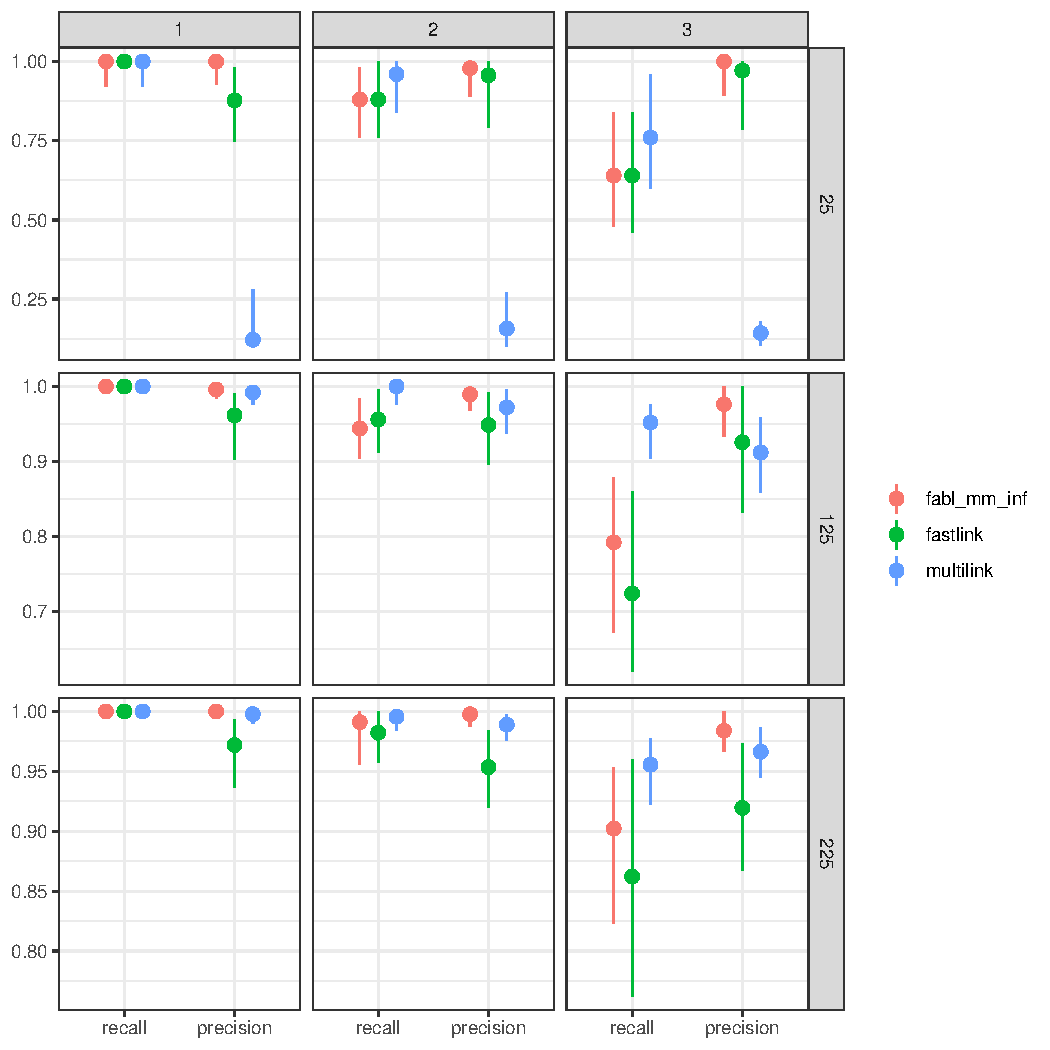
\includegraphics[width=0.8\textwidth]{../Rplots.pdf}
%	\caption{Sadinle Simulation}
%	\label{fig:sadinle}
%\end{figure}

\begin{figure}[t]
	\centering
	\includegraphics[width=0.8\textwidth]{../figures/sadinle_recall.png}
	\caption{Recall for simulations in Section~\ref{sec:simulations}.}
	\label{fig:sadinle-recall}
\end{figure}

\begin{figure}
	\centering
	\includegraphics[width=0.8\textwidth]{../figures/sadinle_precision.png}
	\caption{Precision for simulations in Section~\ref{sec:simulations}.}
	\label{fig:sadinle-precision}
\end{figure}

\begin{figure}
	\centering
	\includegraphics[width=0.8\textwidth]{../figures/sadinle_fmeasure.png}
	\caption{F-Measure for simulations in Section~\ref{sec:simulations}.}
	\label{fig:sadinle-fmeasure}
\end{figure}


In these simulations, standard \texttt{fabl} drastically underperforms, so much so we omit results from the figures below. For each record in $B$ with matching records in $A$, the posterior match probability is split between the two matching records. Due to the randomness of the Gibbs sampler, one of the records occasionally has a posterior probability over 0.5 and is thus identified through the Bayes estimate, but often, both records have posterior probability below 0.5. Under \texttt{vabl}, the posterior probability of the two records is cut precisely in half, and thus \texttt{vabl} did not identify any matching record pairs in any of the simulations. Again, these results are omitted.

We see that \texttt{fastLink} generally has poorer performance than the more complex models at mid to high overlap. In particular, without a post-processing step tailors the scenario where one record in $B$ can match to multiple records in $A$, \texttt{fastLink} tends to produce a large number of false positives, hindering precision, as shown in Figure \ref{fig:sadinle-precision}.

The performance of \texttt{multilink} is more varied. When using substantive prior information, \texttt{multilink} outperforms \texttt{DRL} in terms of overall F-measure in the medium and high overlap settings. However, when the number of matching records pairs is low, \texttt{multilink} underperforms. This may be because the model being fit is more complex, and so it is more difficult to learn the parameters from such few observations. Notably however, the performance of \texttt{multilink} is highly sensitive to prior specification. When using default settings, \texttt{multilink} showed considerably lower recall and precision at all levels of error and overlap.



%The "fabl swap" approach here is also strong. It generally has higher recall, but lower precision. This makes sense, because it doesn't need to consecutive matching algorithim in order to find the "multiple matches", but it also doesn't employ any post processing to clean up erroneous matches. In all simulations, multiple match and fabl swap have similar f-measure. (Not sure exactly how I want to analyze that. In NCVR, there is more of a difference.) 

We see that \texttt{DRL} is a strong alternative to \texttt{multilink} and \texttt{fastLink} in this setting. \texttt{DRL} maintains strong performance even in the low overlap scenario where \texttt{multilink} fails, and outperforms \texttt{fastLink} in terms of F-measure at all levels of error and overlap. We accomplish this through default, uniform priors for the sequence of $\eta_k$ parameters, without needing the informative priors required for \texttt{multilink}. Additionally, the average computation time for 1000 iterations of the Gibbs sampler for \texttt{DRL} was around 30 seconds, while it was around 1000 seconds for \texttt{multilink}. 

\section{Case Study}\label{sec:case-study}

We demonstrate our method on the North Carolina Voter Registration (\texttt{NCVR}) database taken two months apart ~\citep{christen_preparation_2014}. The snapshots are filtered to include only those voters whose details changed over the two-month period, so there are matching records with full agreement on all fields. We use first name, middle name, last name, as string fields, and street address and age as categorical fields. Unique voter registration numbers are provided, however they are known to contain some errors. The \texttt{NCVR} dataset is not publicly available due to sensitive information. However, we have permission to utilize it for publication by its owner.

Using the voter registration numbers, we can see that each file has internal duplication rates of about 1\%. In this analysis, we deduplicate file $B$, and left $A$ with duplicates. In practice, such low amount of internal duplication may not warrant the use of Dirichlet Beta Linkage since \texttt{vabl} is considerably faster. However, we demonstrate here that even with such few internal duplications, \texttt{DBL} is effective at identifying this multiple matches and does not declare too many false matches. 

I compare four approaches: standard \texttt{fabl}, our proposed \texttt{DRL} method, \texttt{fastLink}, and \texttt{fastLink} with the Jaro correction. This task is too large for running \texttt{multilink} in its current implementation in \texttt{R}, and is thus omitted. For \texttt{fastLink}, we use the threshold of 0.5 to declare matches, and for \texttt{fabl} and \texttt{DRL}, we use losses that are equivalent to a threshold of 0.5. Results are in Table \ref{table:ncvr_results}.

\begin{table}[t]
	\centering
	\begin{tabular}{l|rrr}
		method & recall & precision & f\_measure\\
		\hline
		\texttt{DRL} & 0.9891623 & 0.9735309 & 0.9812843\\
		\hline
		\texttt{fabl} & 0.9743739 & 0.9798799 & 0.9771191\\
		%\hline
		%fabl\_swap & 0.9842840 & 0.9420737 & 0.9627164\\
		\hline
		\texttt{fastLink} & 0.9988472 & 0.8494865 & 0.9181321\\
		\hline
		\texttt{fastLink} (with Jaro) & 0.9514490 & 0.9664229 & 0.9588775\\
	\end{tabular}
	\caption{Accuracy results for \texttt{NCVR}, showing the \texttt{DRL} has the highest f-measure.}
	\label{table:ncvr_results}
\end{table}

We see that \texttt{fastLink} without the one-to-one post-processing results in the highest recall, but leads to an undesirable amount of false positives. Since the posterior match probability of each record pair is computed independently, we expect such behavior on large linkage tasks such as this. When we use the Jaro post-processing to achieve a one-to-one matching, we get considerably better results. However, we lose the possibility of identifying cases where one record in $B$ matches to two records in $A$, and we still have worse recall and precision than attained under standard \texttt{fabl}. 

In Figure~\ref{fig:ncvr_thresholds}, we show the show the precision, recall, and F-measure under various choices of match probability thresholds. We see that \texttt{fabl} and \texttt{DRL} produce more refined match probability estimates, allowing the accuracy metrics to vary smoothly across the different thresholds. In contrast, all record pairs of the same agreement pattern under \texttt{fastLink} have the same posterior probability, leading to much a much coarser posterior distribution, leading to more erratic curves. We see that \texttt{fabl} maintains the highest precision at all thresholds, but that \texttt{DRL} is able to identify enough more additional true matches that \texttt{DRL} maintains the highest overall F-measure.
%Overall, we see that \texttt{DRL} has the highest F-measure under all probability thresholds considered, followed by \texttt{fabl}, and then by \texttt{fastLink}.
\begin{figure}[t]
	\centering
	\includegraphics[width=0.9\textwidth]{../figures/ncvr_thresholds}
	\caption{Accuracy metrics for NCVR data at various match probability thresholds. We see that \texttt{DRL} maintains the strongest F-measure for all thresholds considered.}
	\label{fig:ncvr_thresholds}
\end{figure}

Lastly, we note a limitation in using preexisting software for record linkage tasks. In its currently implementation, \texttt{fastLink} allows users to define normalized Levenshtein distance thresholds for coding field comparisons into three discrete levels. In this data however, it is common for a record to contain a middle initial (like ``E"), rather than a full middle name (like ``Elizabeth"). Using Levenshtein distance thresholds, the comparison field for middle name for such a pair of records could coded as a full disagreement, when it should be more reasonably given its own agreement level. Likewise, when two records have a middle initial that happens to match, this is coded as a full agreement, even though it is possible these initials represent different names. In this analysis, 27.6\% of the false matches under \texttt{DRL} at the 0.5 probability threshold included at least one record containing a middle initial rather than middle name. A more careful construction of the comparison vectors is likely to improve results for all methods considered.

\section{Conclusion}

%	\\
%	&= \prod_{k = 1}^K \frac{1}{n_A - (k - 1)} \eta_k  w_{q_k, j} \\
%	&= p\left(Z_{j, k}^{(s+1)}  = q_k |\gamma, \bm{m}^{(s+1)}, \bm{u}^{(s+1)}, \pi^{(s+1)}, Z_{j, k-1} = q_{k-1} \right)


%\subsection{Gibbs Sampler}
%Through MCMC, we are able to sequentially sample the components $Z_{j, k}$ of the matching set $Z_j$. The first match for $B_j$ is made through the same sampler as was used in \cite{kundinger_2023}.
%
%\begin{align}
%	p(Z_{j, 1}|\eta_k) &= \begin{cases}
%		\frac{\eta_k}{n_1}, &  z_{j, 1} \in [n_1], \\
%		1 - \eta_k, & z_{j, 1} = 0;
%	\end{cases} \\
%	\eta_k &\sim \text{Beta}(\alpha_{\eta}, \beta_{\eta})
%\end{align}
%
%In this context, we use the sequence of priors
%\begin{align}
%	p(Z_{j, k}|\eta_k) &= \begin{cases}
%		\frac{\eta_k}{n_{j, k}}, &  z_{j, k} \in N_{j, k}, \\
%		1 - \eta_k, & z_{j, k} = \emptyset;
%		\end{cases} \\
%	\eta_k &\sim \text{Beta}(\alpha_{\eta}, \beta_{\eta})
%\end{align}
%where $N_{j, k}$ is the set of records in $A$ that are available to be matched with $B_j$, and $n_{j, k} = |N_{j, k}| = n_A - (k - 1)$ is the number of such records. 
%
%This sequence of priors leads to the sequence of posteriors
%\begin{align}
%	p(Z_{j, k}|Z_j^{k-1}, \eta_k, \bm{m}, \bm{u}, \gamma) &= \begin{cases}
%		w_{ij}, & z_{j, k} \in N_{j, k}, \\
%		n_{j, k} \frac{1 - \eta_k}{\eta_k}, & z_j = 0;
%	\end{cases} \\
%	\eta_k &\sim \text{Beta}(\alpha_{\eta} + n_k(Z), \beta_{\eta} + n_{k-1}(Z) - n_k(Z))
%\end{align}
%where $n_k(Z) = \sum_{j=1}^{n_B} I( |Z_j| \geq k)$ is the number of records in $B$ that have at least $k$ matches in $A$. Note that $n_0(Z) = n_B$, and that for each $k$, we can view $n_{k-1}{(Z)}$ as a number of trials, and $n_{k}{(Z)}$ as a number of successes. 
%
%This specification induces an extension of \texttt{fabl} with an iterative matching phase. In each iteration of the Gibbs sampler, we sample an initial set of links using $\eta_1$. For each record in $B$ that was found to have a link, we remove the linked record in $A$ from consideration, and then sample another potential link with $\eta_2$. We continue, using $\eta_k$ in the $k^{th}$ matching step, until no new links are found, at which we point the matching phase terminates. The $\bm{\eta}, \bm{m},$ and $\bm{u}$ parameters are estimated based on all of the links identified. Crucially, there is no need to specify a maximum number of links per record, as this estimated through the model.

%\section{Loss Function}
%
%If we assume there are no duplicates in the base file.
%
%In other Bayesian record linkage approaches, researchers have proposed specialized loss functions that match the specific record linkage model. \cite{sadinle_bayesian_2017}
%
%
%To obtain an estimate $\hat{\bm{Z}}$ of the linkage structure, we use the loss functions and Bayes estimate from \cite{sadinle_bayesian_2017}. Since we model the set of matches for each record $B_j$ independently, it is possible for this Bayes estimate to violate transitivity requirements. Formally, all matched sets such that $\hat{Z}_j \cap \hat{Z}_{j'} = \emptyset$ or  $\hat{Z}_j \cap \hat{Z}_{j'} = \hat{Z}_j$ are in concordance with transitivity. In contrast, 
%
%To obtain a Bayes estimate that fulfills the bipartite requirement, we minimize the expected loss subject to the constraint that $\hat{Z}_j \neq \hat{Z}_{j'}$ for all $j \neq j'$. See Supplement \ref{bayes-estimate} for details regarding the initial Bayes estimate and this post-processing procedure.
%
%If we know that there are no duplication in $B$, we can use the same loss function that we used in \texttt{fabl}. Of course, if we know there are no duplications, we can always swap the datasets and use standard \texttt{fabl} instead of the more complicated multiple match. 
%
%If there are potentially duplicates within $B$, then we need a different loss function to preserve transitivity. One idea is a slightly altered version of the I'm using maximal matching sets from \cite{steorts_bayesian_2016}.
%
%$$p(Z_j = q) =  \frac{1}{S}\sum_{s = 1}^S I\left(Z_j^{(s)} = q\right)$$
%
%Maximal matching sets are in conflict if one is a strict (or proper) subset of another. That is, the matching sets $Z_j$ and $Z_{j'}$ are in conflict if $Z_j \subsetneq Z_{j'}$ or $Z_{j'} \subsetneq Z_j$. In such cases, we calculate the total probability for each cluster, given by $|\hat{Z}_j| p(Z_j = q)$, and accept cluster with the highest total probability. This post-processing ensures transitivity. 



%\subsection{Variational Inference}
%There are several reasons why this prior would not be practical through variational inference.
%\begin{itemize}
%	\item Through MCMC, we can sequentially sample all plausible matches for record $B_j$. In variational inference however, we need to estimate the match probability for the joint distribution of ever possible combination of matches. 
%	\item Without hashing, the number of possible combinations is $n_A \choose k$. With hashing, this number is $P^k / k!$ (I think), and would still require some operations at the scale of $n_A \choose k$ when conducting the actual hashing.
%	\item However, this approach might work if using aggressive indexing/filtering.  
%\end{itemize}
%In cases where we know at least one file is duplicate free, we can safely use \texttt{vabl}. However, if we want to be cautious about the potential for duplicates, the multiple match prior under \texttt{fabl} is a good option. 

%\subsection{Comparison to Base Fellegi-Sunter}
%\begin{itemize}
%	\item At the point at which we allow for duplication within and across datasets, one might ask why we don't just use the independent record pair assumption of base Fellegi Sunter
%	\item We have found that standard FS (and its implementation in fastlink) tends to overmatch. Its performance generally improves once you use the Jaro post-processing algorithm to obtain a one-to-one matching
%	\item In this setting, we do not want a one-to-one matching, so we need to take the raw output of FS
%	\item Conceptually, one could modify the Jaro algorithm to allow for one-to-$K$ matchings. However, this would take some work, and it would have the downside of having to prespecify $K$. 
%\end{itemize}

%\subsection{Computational Considerations}
%We can set the maximum number of linkages per record, $K$, or let it be estimated by the model. Setting it ahead of time gives a minor (I would say, negligible) computational advantage over leaving it unrestricted. 
%
%Let $L_k^{(s)}$ be the number of records in $B$ with at least $k$ links in $A$ during iteration $s$ of the Gibbs sampler. Note that $L_0 = n_B$ and $L_1 = n_{12}(Z^{(s)})$ when conducting single matching. The computational complexity of multiple match using MCMC is $\mathcal{O} \left(P \sum_{k=0}^K L_k\right)$.
%
%When $X_1$ is free of duplicates, the multiple match algorithm makes a second attempt at matching, which has complexity $ \left(P L_1 \right)$. This is a minor addition of computation time, but gives the added security of identifying duplicates. It may be a nice option just to use when you're not sure!

%\section{Preliminary Findings}
%The comparisons are not quite striaghtforward, so I'll have to be creative with the best way to present the findings. Here's an overview:
%\begin{itemize}
%	\item \texttt{multilink} allows the user to set the maximum number of records in each dataset that can form part of a cluster of matching records. If this number is mispecified, results are poor.
%	\item When there are sufficiently many matches to properly estimate the $m$ parameters, fabl with multiple match outperforms base FS. 
%	\item When there are few matches in the data set, fabl drastically overmatch. Basically, the algorithm just keeps identifying matches, muddying up the $m$ distribution, and everything deteriorates from there. 
%	\item This behavior can be ameliorated by preventing the algorithm from overmatching. Two options:
%	\begin{itemize}
%		\item Set $K$, a maximum number of matches per record. This works well, and is more robust to misspecification than the maximum cluster size in multilink.
%		\item Use informative priors on each $\eta_k \sim \text{Beta}(\alpha_{\eta}, \beta_{\eta_k})$. I have had good results with $\beta_{\eta_k} = k^2$ and $\beta_{\eta_k} = k^3$. Note that if this penalty prior takes the general form $\beta_{\eta_k} = k^{\tau}$, we attain fabl at $\tau = \infty$, and conceptually, $\tau$ can be estimated from the data or optimized through cross validation. 
%	\end{itemize}
%\end{itemize}
%
%\section{Simulations}
%
%We demonstrate the accuracy of the multiple match approach at various levels of overlap between files and errors between matching records through an adaptation of the simulation study from \cite{sadinle_bayesian_2017} and \cite{kundinger_2023}. 
%
%For each simulation, we construct two data files $A$ and $B$ such that there are in which there are 25, 125, or 225 records in $B$ that have matching records in $A$. The matching record in $A$ exhibits 1, 2, or 3 errors accross the five fields used for linkage. Then, every record in $A$ that has a matching record in $B$ is duplicated, such that each simulation has 50, 250, or 450 matching record pairs in total. We use uniform priors for the $\bm{m}$ and $\bm{u}$, with $\alpha_{fl} = \beta_{fl} = 1$ for all $f$ and $l$. We use uniform priors for $\pi$ for standard \texttt{fabl}, and also uniform priors for each $\eta_k$ for multiple match. \brian{We correctly specify the prior for multilink. (Need to write provide more description of model to make this succinct)} We run the Gibbs sampler for 1000 iterations, and discard the first 100 as burn-in.
%
%In these simulations, standard \texttt{fabl} drastically under performs, so much so that results are omitted from the graph. For each record in $B$ with matching records in $A$, the posterior match probability is split between the two matching records. Due to the randomness of the Gibbs sampler, one of the records occassionally has a posterior probability over 0.5 and is thus identified through the Bayes estimate, but often, both records have posterior probability below 0.5. In through \texttt{vabl}, the posterior probability of the two records is cut precisely in half, and thus \texttt{vabl} did not identify any matching record pairs in any of the simulations.
%
%The performance of \texttt{multilink} is more varied. When there is a moderate or high amount of matching records, \texttt{multilink} performs comparably with multiple match. However, in the setting where the number of matching records is low, \texttt{multilink} under performs. This may be because the model being fit is more complex, and so it is difficult to learn the parameters from such few observations. Noteably however, the performance of \texttt{multilink} is highly sensitive to prior specification. In FIGURE (to be added), we show accuracy suffers under various forms of mispecification.
%
%The "fabl swap" approach here is also strong. It generally has higher recall, but lower precision. This makes sense, because it doesn't need to consecutive matching algorithim in order to find the "multiple matches", but it also doesn't employ any post processing to clean up erroneous matches. In all simulations, multiple match and fabl swap have similar f-measure. (Not sure exactly how I want to analyze that. In NCVR, there is more of a difference.) 
%
%We see that multiple match is a strong alternative to multiple match in this setting. In particular, the average computation time for 1000 iterations of the Gibbs sampler for multiple match was around 30 seconds, while it was around 1000 seconds for \texttt{multiple match}. 
%
%\begin{figure}[t]
%	\centering
%	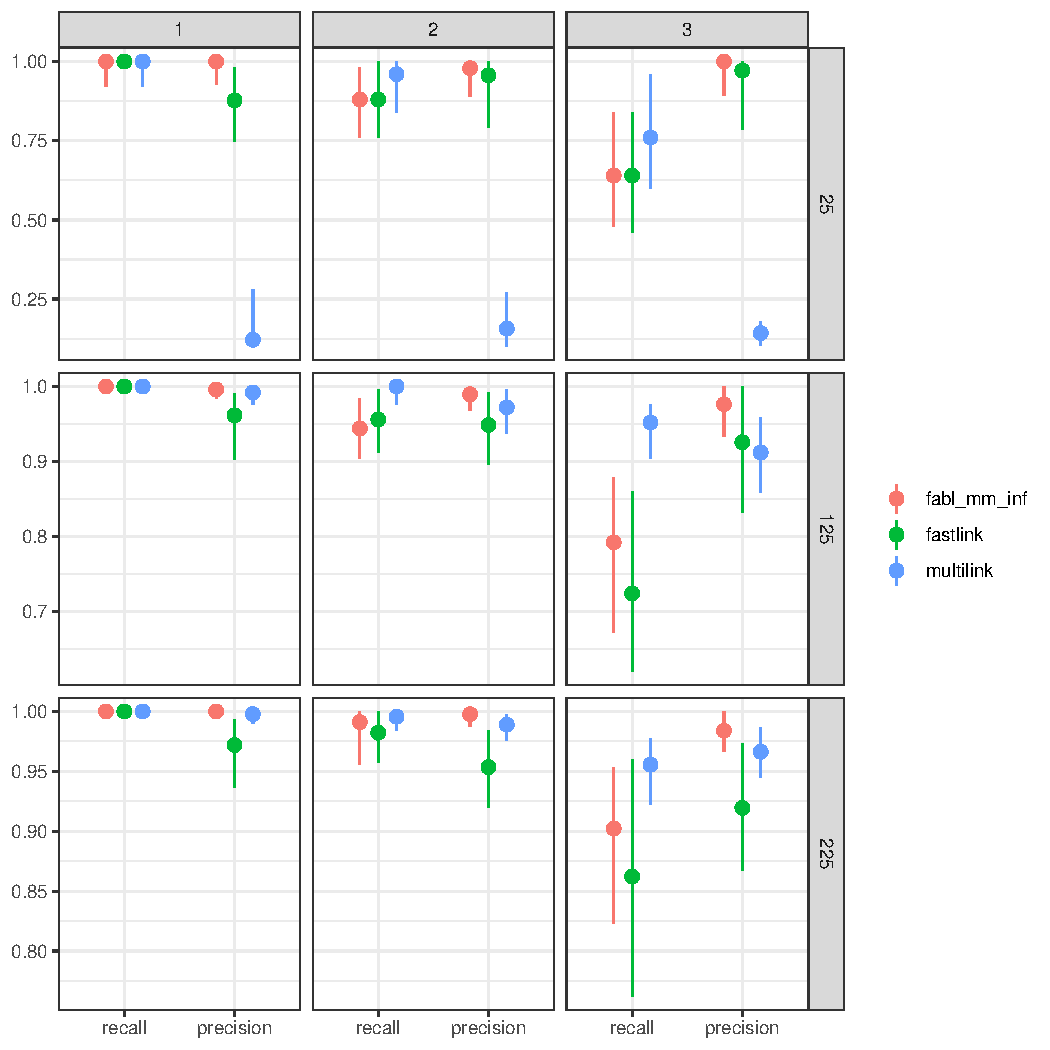
\includegraphics[width=0.8\textwidth]{../Rplots.pdf}
%	\caption{Sadinle Simulation}
%	\label{fig:sadinle}
%\end{figure}
%
%
%NOTE: I've included fastlink (without Jaro) in this image for the time being. However, there is currently no way through fastlink to produce estimates that respect the 2-to-1 matchings while enforcing transitivity. 
%


%We conduct linkage when matching records exhibit 1, 2, and 3 errors across the four fields, and when there are 25, 125, and 225 records in $B$ that have matching records in $A$. To test  Under each of these settings, we use 100 pairs of simulated data files in order to obtain uncertainty quantification on our performance metrics.

%The simulations employ a collection of synthetic data files with varying amounts of error and overlap (the number of records in common across files). Following methods proposed by \cite{christen_pudjijono2009} and \cite{christen_vatsalan2013}, clean records are first simulated from frequency tables for first name, last name, age, and occupation in Australia. Fields are then chosen for distortion uniformly at random. Names are subject to string insertions, deletions and substitutions, as well as common keyboard, phonetic, and optical recognition errors. Age and occupation are distorted through keyboard errors and missingness. These synthetic data files are available in the supplement to \cite{sadinle_bayesian_2017}.
%
%We create comparison vectors according to the default settings of the \texttt{compareRecords} function from the \texttt{BRL} package, shown in Table \ref{Tab:sadinle_simulation_cutoffs}. Each simulation identifies matched individuals between two data files, each with 500 records. We conduct linkage when matching records exhibit 1, 2, and 3 errors across the four fields, and when there are 50, 250, and 450 individuals in common across data files. Under each of these settings, we use 100 pairs of simulated data files in order to obtain uncertainty quantification on our performance metrics. We use uniform priors for the $\bm{m}$, $\bm{u}$, and $\pi$ parameters, with $\alpha_{fl} = \beta_{fl} = 1$ for all $f$ and $l$. We run the Gibbs sampler for 1000 iterations, and discard the first 100 as burn-in. We calculate Bayes estimates $\hat{\bm{Z}}$ of the linkage structure using the  loss function and post-processing procedure described in Supplement \ref{bayes-estimate}. Traceplots for parameters of interest for one example simulation are provided in Supplement \ref{app:appendix-sim}; they show no obvious concern over MCMC convergence. We also replicate this simulation allowing \texttt{fabl} to leave some components of the linkage structure undetermined and left for clerical review; those results are in Supplement \ref{partial}.


%Show accuracy under various settings of maximum cluster size for different algorithms. Recall will fall very quickly for \texttt{fabl}. Since we can't use Jaro, precision for \texttt{fastLink} will be poor.  Multilink may be very dependent on correctly specifying $K$. This multiple match approach should remain strong in all settings. 

\pagebreak
\bibliographystyle{agsm}
\bibliography{biblio}

\pagebreak

\section{Appendix}
\label{sec:appendix}

\subsection{Derivation of Sequential Sampler}\label{app:sequential-sampler}
We now provide the derivation of the sequential sampler, following the argument presented in Section \ref{sec:joint-distribution}. Suppose $B_j$ has been linked to $k$ records in $A$. Let $Z_{j, -k} = (Z_{j, 1}, \ldots, Z_{j, k-1})$ denote the vector of records already linked to $B_j$. When $B_j$ has no additional link in $A$, the contribution to the likelihood is a product of the $u$ parameters for all remaining records. That is, 
\begin{align}
	p(\Gamma_{.j}| \bm{m}, \bm{u}, \pi, Z_{j, k} = \emptyset, Z_{j, -k} = q_{-k}) = \prod_{i \notin Z_{j, -k}} \prod_{f=1}^{F}\prod_{l=1}^{L_f} u_{fl}^{I(\gamma_{ij}^f = l)I_{obs}(\gamma_{ij}^f)} = c_{Z_{j, -k}}.
\end{align}

When $Z_{j, k} = q_k$ for some $q_k > 0$, we have
\begin{align}
	p(\Gamma_{.j}| \bm{m}, \bm{u}, \pi,  Z_{j, k} = q_k, Z_{j, -k} = q_{-k}) &=\prod_{f=1}^{F}\prod_{l=1}^{L_f} m_{fl}^{I(\gamma_{q_k, j}^f = l)I_{obs}(\gamma_{q_k, j}^f)}  \prod_{i \notin (q_{-k}, q_k)}\prod_{f=1}^{F}\prod_{l=1}^{L_f} u_{fl}^{I(\gamma_{ij}^f = l)I_{obs}(\gamma_{ij}^f)} \\
	&=\prod_{f=1}^{F}\prod_{l=1}^{L_f} \left(\frac{m_{fl}}{u_{fl}} \right)^{I(\gamma_{q_k, j}^f = l)I_{obs}(\gamma_{q_k, j}^f)}  \prod_{i \notin (Z_{j, -k}}\prod_{f=1}^{F}\prod_{l=1}^{L_f} u_{fl}^{I(\gamma_{ij}^f = l)I_{obs}(\gamma_{ij}^f)} \\
	&= c_{Z_{j, -k}} w_{q_k, j}
\end{align}
To obtain the posterior, we multiply by the prior in (\ref{eqn:sequential_prior}). The posterior distribution this is given by
\begin{align}\label{eqn:sequential-posterior-full}
	p(Z_{j, k} = q_k|Z_{j, k-1}, \eta_k, \bm{m}, \bm{u}, \gamma) &=
	\frac{\left(\frac{\eta_k}{n_A - (k - 1)}c_{Z_{j, -k}} w_{q_k, j}\right)^{I(q_k \in N_{j, k})} + \left(c_{Z_{j, -k}}(1 - \eta_k)\right)^{I(q_k = \emptyset)}}{\frac{\eta_k}{n_A - (k - 1)}c_{Z_{j, -k}} \sum_{i \notin Z_{j, -k}} w_{ij} + c_{Z_{j, -k}}(1 - \eta_k)} \\
	&=
	\frac{\left(\frac{\eta_k}{n_A - (k - 1)}w_{q_k, j}\right)^{I(q_k \in N_{j, k})} + (1 - \eta_k)^{I(q_k = \emptyset)}}{\frac{\eta_k}{n_A - (k - 1)}\sum_{i \notin Z_{j, -k}} w_{ij} +(1 - \eta_k)} \\
	&\propto \begin{cases}
		\frac{\eta_k}{n_A - (k - 1)} w_{q_k, j}, & q_k \in N_{j, k}, \\
		1 - \eta_k, & q_k= \emptyset.
	\end{cases}
\end{align}
Importantly, the constant $c_{Z_{j, -k}}$ is not found in the final expression because the probability mass associated with every potential value for $Z_j$ shares the same $c_{Z_{j, -k}}$. This does not occur due to proportionality. 


%\subsection{Extended Proof} \label{app:extended-proof}
%\begin{align*}
%	p\left(Z_j  = q |\gamma, \bm{m}, \bm{u}, \pi\right) &\propto \frac{(n_A - |q|)!|q|!}{n_A!} \pi_{|q|} \prod_{i \in q} w_{ij} \\
%	&= \prod_{c = 1}^{|q|} \frac{1}{n_A - (c + 1)} (1 - \eta_{|q|+1}) |q|!\prod_{c = 1}^{|q|} \eta_{|q|} \prod_{c = 1}^{|q|} w_{q_c, j} \\
%	&= (1 - \eta_{|q|+1}) |q|!\prod_{c = 1}^{|q|} \frac{\eta_{|q|} }{n_A - (c + 1)}  \prod_{c = 1}^{|q|} w_{q_c, j} \\
%	&= p(Z_{j, |q|+1} = \emptyset| \eta_{|q|})|q|! \prod_{c = 1}^{|q|} p(Z_{j, c} = q_c|\eta_c) p(\Gamma_{.j}| \bm{m}, \bm{u}, \bm{\eta}, q_c \in Z_j) \\
%	&\propto p(Z_{j, |q|+1} = \emptyset | \Gamma_{.j}, \bm{m}, \bm{u}, \bm{\eta}) |q|!\prod_{c = 1}^{|q|} p(Z_{j, c} = q_c|\Gamma_{.j}, \bm{m}, \bm{u}, \bm{\eta}).
%\end{align*}
%
%\begin{align}
%	p\left(Z_j  = q|\gamma, \bm{m}, \bm{u}, \pi \right) &= \frac{\frac{(n_A - |q|)! |q|!}{n_A!} \pi_{|q|} c_j \prod_{i \in q} w_{ij}}{\sum_{h \in \mathcal{Z}} \frac{(n_A - |h|)! |h|!}{n_A!} \pi_{|h|} c_j \prod_{i \in h} w_{ij}} \\
%	&= \frac{\frac{(n_A - |q|)! |q|!}{n_A!} \pi_{|q|} \prod_{i \in q} w_{ij}}{\sum_{h \in \mathcal{Z}} \frac{(n_A - |h|)! |h|!}{n_A!} \pi_{|h|} \prod_{i \in h} w_{ij}} \\
%	&\propto \frac{(n_A - |q|)! |q|!}{n_A!} \pi_{|q|} \prod_{i \in q} w_{ij}
%\end{align}
%
%\begin{align}
%	\prod_{c = 1}^{|q|} p\left(Z_{j, c} = q_c|\gamma, \bm{m}, \bm{u}, \eta_c, Z_{j, c-1} \right) &=  (1 - \eta_{|q|+1}) |q|!\prod_{c = 1}^{|q|} \frac{\eta_{|q|} }{n_A - (c + 1)}  \prod_{c = 1}^{|q|} w_{q_c, j}
%\end{align}


\subsection{Efficient Sequential Sampling Details}
%Following \cite{kundinger_2023} we use hashing to reduce the computational complexity of the Gibbs sampler. Since each component $\gamma_{ij}^f$ of the comparison vector is discrete, there are only finitely many possible realizations of the comparison vector $\gamma_{ij}$. Let $P$ be the number of unique agreement patterns observed in $\Gamma$. This number is bounded above by $P^{*} =  \prod_{f=1}^F (L_f + 1)$, where the addition of 1 to $L_f$ for each field accounts for the possibility of missing values. This upper bound does not scale with $n_1$ or $n_2$, but rather is determined by $F$ and $L_f$.  
%
%We adopt a hashing function to map the $P$ unique agreement patterns present in the comparison vectors to the integers in $[P]$. Let
%\begin{equation}
%	\label{eq:hashfunc}
%	h_f^{(i,j)} = I_{obs}( \gamma_{ij}^f) 2^{\gamma_{ij}^f + I(f>1) \times \sum_{e=1}^{f-1}(L_{e} - 1)}
%\end{equation}
%denote a hashed value for field $f$ for record pair $(i,j)$. Summing over the fields for the agreement pattern of record pair $(i,j)$ gives the hash value $h^{(i,j)}=\sum_{f=1}^Fh_f^{(i,j)}$. We enumerate the unique hashed agreement patterns from $1$ to $P$. Denote each agreement pattern as $h_p=(h_p^1,\dots,h_p^F)$, so that when record pair $(i,j)$ exhibits agreement pattern $p$, we write $\gamma_{ij}=h_p$.  Collect the agreement patterns as $\mathcal{P}=\{h_p\mid p\in[P]\}$.
%
%Let $e(h_p)$ denote the $\sum_{f=1}^FL_f$ length vector in which the $l + \sum_{k=1}^{f-1} L_k$ component is 1 when $h_p^f = l$, and 0 otherwise. Observe that $e(h_p)$ represents a long version of $h_p$, which is useful for computational purposes. Let $N_{p_j}=\sum_{i=1}^{n_2}I(\gamma_{ij}=h_p)$ denote the number of records in $X_1$ with which record $j$ in $X_2$ has agreement pattern $p$. Collect these counts in $\mathcal{N}=\{N_{p_j}\mid j\in[n_2], p\in[P]\}.$ Let $N_p=\sum_{j=1}^{n_2}N_{p_j}$ denote the total number of record pairs with agreement pattern $p$. Finally, let $r_{p_j}=\{i\in[n_1]\mid \gamma_{ij}=h_p\}$ be the set of records in $X_1$ with which record $j$ in $X_2$ has agreement pattern $p$, and collect these sets as $\mathcal{R}=\{r_{p_j}\mid p\in[P], j\in[n_2]\}$. 
%
%The set $\tilde{\bGamma}=\{ \mathcal{P}, \mathcal{R},\mathcal{N}\}$ fully characterizes the information in $\bGamma$ at a reduced storage cost. In particular, by letting 
%\[
%m_p = \prod_{f=1}^F\prod_{l=1}^{L_f} m_{fl}^{I(h_p^{f}=l)I_{obs}(h_p^{f})}
%\]
%and
%\[
%u_p = \prod_{f=1}^F\prod_{l=1}^{L_f} u_{fl}^{I(h_p^{f}=l)I_{obs}(h_p^{f})},
%\]
%the likelihood function in \eqref{eqn:likelihood} can be written as
%\begin{equation}
%	\label{eq:likelihoodhash}
%	\mathcal{L}(Z, m,u\mid\tilde{\Gamma})=\prod_{j=1}^{n_2}\prod_{p=1}^{P}\prod_{i\in r_{p_j}}m_p^{I(Z_j=i)}u_{p}^{I(Z_j\neq i)}.
%\end{equation} 
\end{document}
